\documentclass[border=3pt]{standalone}
% Preâmbulo compartilhado pelos diagramas TikZ da aula 7 (Filtros Não Paramétricos)
\usepackage[T1]{fontenc}
\usepackage[utf8]{inputenc}
\usepackage{lmodern}
\usepackage{amsmath}
\usepackage{xcolor}
\usepackage{tikz}
\usetikzlibrary{arrows.meta,angles,quotes,decorations.pathmorphing,calc,
                positioning,shapes.geometric,shapes.misc,backgrounds,fit,
                math}

% Paleta (mesma dos SVGs originais)
\definecolor{dblue}{HTML}{2A5B8C}
\definecolor{dorange}{HTML}{B3541E}
\definecolor{dgreen}{HTML}{4A7C59}
\definecolor{dred}{HTML}{9C4B4B}
\definecolor{dcream}{HTML}{F4F1EA}
\definecolor{dshade}{HTML}{DDD7C9}

% Função gaussiana (não normalizada por padrão de escala visual)
\pgfmathdeclarefunction{gauss}{3}{%
  \pgfmathparse{1/(#3*sqrt(2*pi))*exp(-((#1-#2)^2)/(2*#3^2))}%
}

% Estilos comuns (prefixo d... para não colidir com chaves internas do pgf)
\tikzset{
  >={Stealth[length=2mm]},
  dguide/.style={gray!55, dashed, line width=0.4pt},
  daxis/.style={gray!60, line width=0.7pt, ->},
  dbody/.style={fill=black!3, draw=black!80, line width=1pt},
  dacc/.style={draw=dblue, line width=1pt},
  dlbl/.style={black!55, font=\small},
  dsub/.style={black!45, font=\footnotesize},
  dstate/.style={circle, draw=black!80, fill=dcream, line width=1pt,
                 minimum size=17mm, font=\large, inner sep=1pt},
  dobs/.style={circle, draw=black!80, fill=dshade, line width=1pt,
               minimum size=14mm, font=\large, inner sep=1pt},
  dbox/.style={rounded corners=2pt, draw=black!80, fill=dcream, line width=1pt,
               align=center, inner sep=6pt},
  dop/.style={circle, draw=black!80, fill=white, line width=1pt,
              minimum size=6mm, inner sep=0pt, font=\small},
  dtrans/.style={->, dblue, line width=1pt},
  dmeas/.style={->, dorange, line width=1pt},
  dcurve/.style={line width=1pt, dblue},
  dcurveb/.style={line width=1.4pt, dorange},
}

\begin{document}
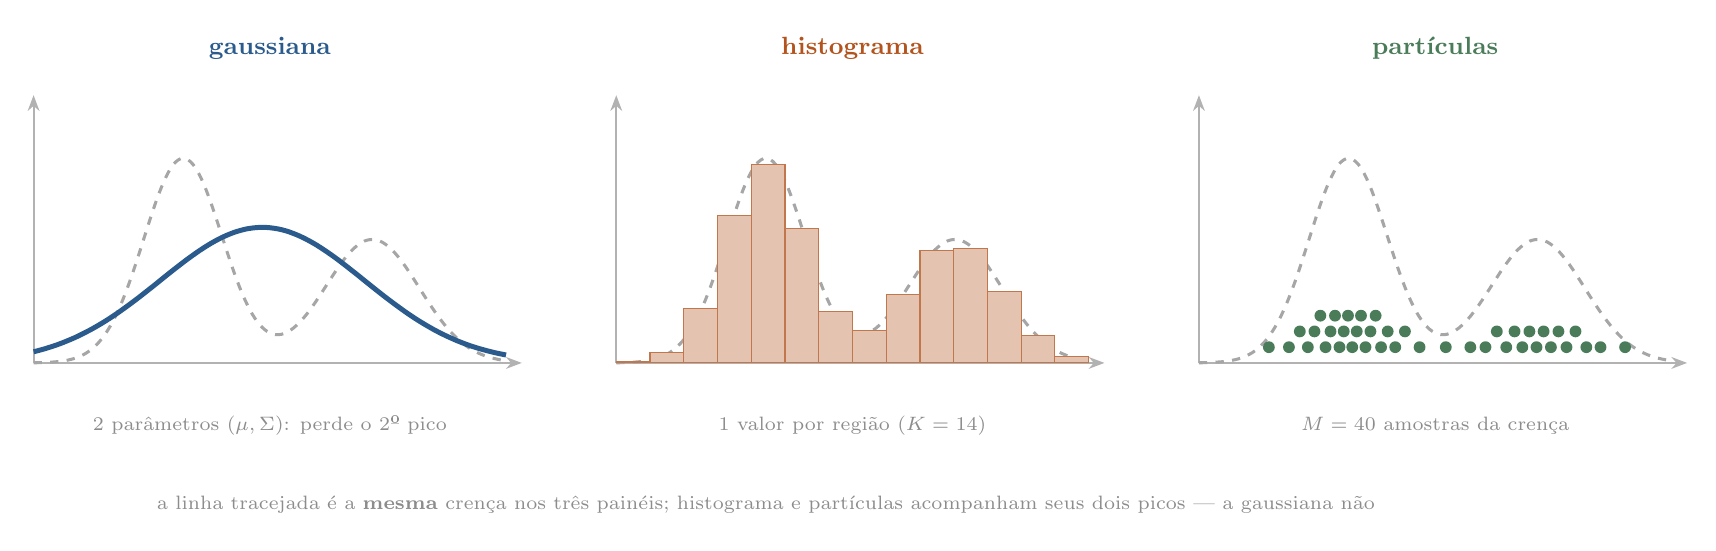
\begin{tikzpicture}[x=1cm,y=1cm]
  \newcommand{\eixo}{\draw[daxis] (0,0) -- (6.2,0); \draw[daxis] (0,0) -- (0,3.4);}
  \newcommand{\verdadeira}{\draw[black!35, line width=1.1pt, dashed] plot[smooth] coordinates {(0.000,0.002) (0.075,0.003) (0.150,0.006) (0.225,0.010) (0.300,0.016) (0.375,0.025) (0.450,0.039) (0.525,0.059) (0.600,0.089) (0.675,0.129) (0.750,0.185) (0.825,0.258) (0.900,0.352) (0.975,0.470) (1.050,0.613) (1.125,0.782) (1.200,0.976) (1.275,1.190) (1.350,1.420) (1.425,1.655) (1.500,1.888) (1.575,2.105) (1.650,2.294) (1.725,2.445) (1.800,2.548) (1.875,2.597) (1.950,2.587) (2.025,2.521) (2.100,2.402) (2.175,2.238) (2.250,2.039) (2.325,1.818) (2.400,1.587) (2.475,1.357) (2.550,1.139) (2.625,0.940) (2.700,0.768) (2.775,0.624) (2.850,0.512) (2.925,0.431) (3.000,0.381) (3.075,0.359) (3.150,0.364) (3.225,0.393) (3.300,0.443) (3.375,0.512) (3.450,0.596) (3.525,0.694) (3.600,0.802) (3.675,0.917) (3.750,1.033) (3.825,1.148) (3.900,1.257) (3.975,1.355) (4.050,1.438) (4.125,1.503) (4.200,1.547) (4.275,1.567) (4.350,1.563) (4.425,1.535) (4.500,1.484) (4.575,1.412) (4.650,1.323) (4.725,1.221) (4.800,1.108) (4.875,0.991) (4.950,0.872) (5.025,0.756) (5.100,0.645) (5.175,0.542) (5.250,0.448) (5.325,0.365) (5.400,0.292) (5.475,0.231) (5.550,0.179) (5.625,0.137) (5.700,0.103) (5.775,0.076) (5.850,0.056) (5.925,0.040) (6.000,0.028)};}
  \begin{scope}
    \eixo \verdadeira \node[font=\small\bfseries, dblue] at (3,4.0) {gaussiana};
    \draw[dblue, line width=1.8pt] plot[smooth] coordinates {(0.000,0.142) (0.075,0.161) (0.150,0.182) (0.225,0.206) (0.300,0.231) (0.375,0.259) (0.450,0.290) (0.525,0.322) (0.600,0.358) (0.675,0.396) (0.750,0.436) (0.825,0.479) (0.900,0.524) (0.975,0.572) (1.050,0.622) (1.125,0.675) (1.200,0.729) (1.275,0.785) (1.350,0.842) (1.425,0.901) (1.500,0.960) (1.575,1.020) (1.650,1.081) (1.725,1.141) (1.800,1.200) (1.875,1.258) (1.950,1.315) (2.025,1.369) (2.100,1.422) (2.175,1.471) (2.250,1.517) (2.325,1.559) (2.400,1.597) (2.475,1.630) (2.550,1.659) (2.625,1.682) (2.700,1.701) (2.775,1.713) (2.850,1.720) (2.925,1.722) (3.000,1.717) (3.075,1.707) (3.150,1.692) (3.225,1.671) (3.300,1.644) (3.375,1.613) (3.450,1.577) (3.525,1.537) (3.600,1.493) (3.675,1.445) (3.750,1.394) (3.825,1.341) (3.900,1.285) (3.975,1.227) (4.050,1.168) (4.125,1.109) (4.200,1.048) (4.275,0.988) (4.350,0.928) (4.425,0.869) (4.500,0.811) (4.575,0.755) (4.650,0.700) (4.725,0.646) (4.800,0.595) (4.875,0.546) (4.950,0.500) (5.025,0.456) (5.100,0.414) (5.175,0.375) (5.250,0.339) (5.325,0.305) (5.400,0.273) (5.475,0.244) (5.550,0.217) (5.625,0.193) (5.700,0.171) (5.775,0.151) (5.850,0.132) (5.925,0.116) (6.000,0.101)};
    \node[dsub, font=\scriptsize, align=center] at (3,-0.8) {2 parâmetros ($\mu,\Sigma$): perde o 2º pico};
  \end{scope}
  \begin{scope}[shift={(7.4,0)}]
    \eixo \verdadeira \node[font=\small\bfseries, dorange] at (3,4.0) {histograma};
    \fill[dorange!35, draw=dorange!80, line width=0.4pt] (0.000,0) rectangle (0.429,0.012);
    \fill[dorange!35, draw=dorange!80, line width=0.4pt] (0.429,0) rectangle (0.857,0.128);
    \fill[dorange!35, draw=dorange!80, line width=0.4pt] (0.857,0) rectangle (1.286,0.692);
    \fill[dorange!35, draw=dorange!80, line width=0.4pt] (1.286,0) rectangle (1.714,1.867);
    \fill[dorange!35, draw=dorange!80, line width=0.4pt] (1.714,0) rectangle (2.143,2.519);
    \fill[dorange!35, draw=dorange!80, line width=0.4pt] (2.143,0) rectangle (2.571,1.710);
    \fill[dorange!35, draw=dorange!80, line width=0.4pt] (2.571,0) rectangle (3.000,0.648);
    \fill[dorange!35, draw=dorange!80, line width=0.4pt] (3.000,0) rectangle (3.429,0.416);
    \fill[dorange!35, draw=dorange!80, line width=0.4pt] (3.429,0) rectangle (3.857,0.871);
    \fill[dorange!35, draw=dorange!80, line width=0.4pt] (3.857,0) rectangle (4.286,1.433);
    \fill[dorange!35, draw=dorange!80, line width=0.4pt] (4.286,0) rectangle (4.714,1.456);
    \fill[dorange!35, draw=dorange!80, line width=0.4pt] (4.714,0) rectangle (5.143,0.907);
    \fill[dorange!35, draw=dorange!80, line width=0.4pt] (5.143,0) rectangle (5.571,0.346);
    \fill[dorange!35, draw=dorange!80, line width=0.4pt] (5.571,0) rectangle (6.000,0.081);
    \node[dsub, font=\scriptsize, align=center] at (3,-0.8) {1 valor por região ($K=14$)};
  \end{scope}
  \begin{scope}[shift={(14.8,0)}]
    \eixo \verdadeira \node[font=\small\bfseries, dgreen] at (3,4.0) {partículas};
    \fill[dgreen] (0.888,0.200) circle (0.075);
    \fill[dgreen] (1.143,0.200) circle (0.075);
    \fill[dgreen] (1.281,0.400) circle (0.075);
    \fill[dgreen] (1.383,0.200) circle (0.075);
    \fill[dgreen] (1.467,0.400) circle (0.075);
    \fill[dgreen] (1.542,0.600) circle (0.075);
    \fill[dgreen] (1.608,0.200) circle (0.075);
    \fill[dgreen] (1.671,0.400) circle (0.075);
    \fill[dgreen] (1.728,0.600) circle (0.075);
    \fill[dgreen] (1.785,0.200) circle (0.075);
    \fill[dgreen] (1.839,0.400) circle (0.075);
    \fill[dgreen] (1.893,0.600) circle (0.075);
    \fill[dgreen] (1.947,0.200) circle (0.075);
    \fill[dgreen] (2.004,0.400) circle (0.075);
    \fill[dgreen] (2.058,0.600) circle (0.075);
    \fill[dgreen] (2.115,0.200) circle (0.075);
    \fill[dgreen] (2.178,0.400) circle (0.075);
    \fill[dgreen] (2.244,0.600) circle (0.075);
    \fill[dgreen] (2.313,0.200) circle (0.075);
    \fill[dgreen] (2.397,0.400) circle (0.075);
    \fill[dgreen] (2.493,0.200) circle (0.075);
    \fill[dgreen] (2.616,0.400) circle (0.075);
    \fill[dgreen] (2.802,0.200) circle (0.075);
    \fill[dgreen] (3.135,0.200) circle (0.075);
    \fill[dgreen] (3.447,0.200) circle (0.075);
    \fill[dgreen] (3.639,0.200) circle (0.075);
    \fill[dgreen] (3.783,0.400) circle (0.075);
    \fill[dgreen] (3.903,0.200) circle (0.075);
    \fill[dgreen] (4.008,0.400) circle (0.075);
    \fill[dgreen] (4.107,0.200) circle (0.075);
    \fill[dgreen] (4.197,0.400) circle (0.075);
    \fill[dgreen] (4.287,0.200) circle (0.075);
    \fill[dgreen] (4.377,0.400) circle (0.075);
    \fill[dgreen] (4.470,0.200) circle (0.075);
    \fill[dgreen] (4.566,0.400) circle (0.075);
    \fill[dgreen] (4.668,0.200) circle (0.075);
    \fill[dgreen] (4.782,0.400) circle (0.075);
    \fill[dgreen] (4.920,0.200) circle (0.075);
    \fill[dgreen] (5.100,0.200) circle (0.075);
    \fill[dgreen] (5.412,0.200) circle (0.075);
    \node[dsub, font=\scriptsize, align=center] at (3,-0.8) {$M=40$ amostras da crença};
  \end{scope}
  \node[dsub, font=\scriptsize, align=center, text width=18cm] at (9.3,-1.8) {a linha tracejada é a \textbf{mesma} crença nos três painéis; histograma e partículas acompanham seus dois picos --- a gaussiana não};
\end{tikzpicture}
\end{document}
